\section{Ex2.10 Throwing two dice}\label{sec:Throwing_two_dice}

\subsection{Testo esercizio}
Lanciare una coppia di dadi a sei facce e sommarne il numero di ciascuno dei dadi: 
$$Z=X1+X2$$ dove $Z$ è la somma dei risultati dei dadi 1, $X1$, e 2, $X2$. Eseguire 
questo esperimento molte volte $(N)$, e trovarne la \textit{media} e la 
\textit{deviazione standard}.
La media,$\langle Z\rangle$ è stimata da:
$$\langle Z\rangle=\frac{1}{N}\sum_{j=1}^{N}Z_j $$ 

la deviazione standard, $\Delta Z$, invece:
$$\Delta Z=\frac{1}{N-1}\sum_{j=1}^{N}\left(Z_j-Z\right)^2 $$

\begin{itemize}
    \item[a)] Scrivere una funzione che restituisce una matrice di $N$ valori per $Z$.
    
    \item[b)] Scrivere una funzione che restituisce una stima della media di una matrice 
    $Z$ utilizzando la formula fornita.

    \item[c)] Scrivere una funzione che restituisce una stima della deviazione standard 
    di una matrice $Z$ utilizzando la formula fornita.
    
    \item[d)] Trova la media e la deviazione standard per $N=100$ lanci di due dadi.
\end{itemize}

\subsection{Svolgimento}
L'esercizio è stato molto divertente. Alcuni problemi sono sorti per colpa di 
un errore di stampa nella formula, che \verb*|google.it| ha prontamente 
risolto. Questo esercizio mi ha anche permesso di creare tabelle con 
associazione di dati, tipo percentuale e conteggio di ogni singola somma 
($1-12$)
\pagebreak

\subsection{Risultati}
\subsubsection{Grafico}
\begin{figure}[h]
    \centering
    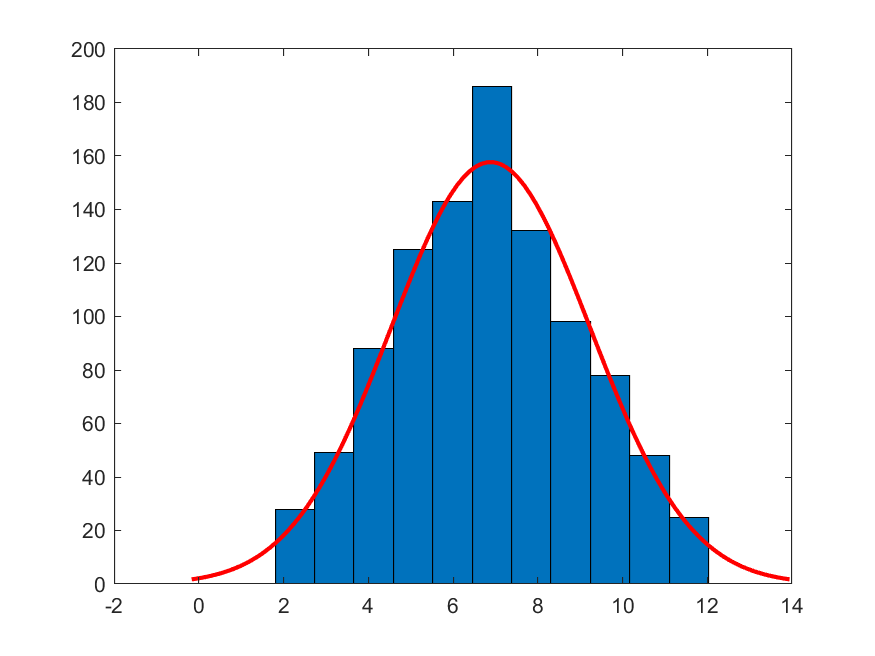
\includegraphics[width=0.7\linewidth]{cap/Elementary/img/script210}
    \GraphCap{Lancio dei dadi}
    \label{fig:script210}
\end{figure}
\subsubsection{Tabella}
\providecommand*{\thead}[1]{\multicolumn{1}{c}{\bfseries #1}}%
\providecommand*{\unitHead}[1]{\multicolumn{1}{c}{\si{#1}}}%

\begin{table}[h]%
\centering%
\begin{tabular}{S[table-format=-1.3]S[table-format=-1.3]S[table-format=-1.3]}%
\toprule%
\thead{throwDice}&\thead{GroupCount}&\thead{Percent}\\
\toprule%
2.00	&	28.00	&	2.80 \\%
3.00	&	49.00	&	4.90 \\%
4.00	&	88.00	&	8.80 \\%
5.00	&	125.00	&	12.50 \\%
6.00	&	143.00	&	14.30 \\%
7.00	&	186.00	&	18.60 \\%
8.00	&	132.00	&	13.20 \\%
9.00	&	98.00	&	9.80 \\%
10.00	&	78.00	&	7.80 \\%
11.00	&	48.00	&	4.80 \\%
12.00	&	25.00	&	2.50 \\%
\bottomrule%
\end{tabular}%
\caption{table210}%
\label{tab:table210}%
\end{table}%
\pagebreak

\subsection{Codice esercizio}
\lstinputlisting[caption = {Funzione ThrowingTwoDice},
linerange={32-42}]
{cap/Elementary/src/function/ThrowingTwoDice.m}

%\lstinputlisting[caption = {Funzione myMean}, label={lst:MyMean}]
%{cap/Elementary/src/function/myMean.m}

%\lstinputlisting[caption = {Funzione myStd}]
%{cap/Elementary/src/function/myStd.m}

\lstinputlisting[title = {Script Ex2.10},
linerange={3-16}]
{cap/Elementary/src/script/script210.m}
